% Created by tikzDevice version 0.10.1 on 2019-04-11 12:59:42
% !TEX encoding = UTF-8 Unicode
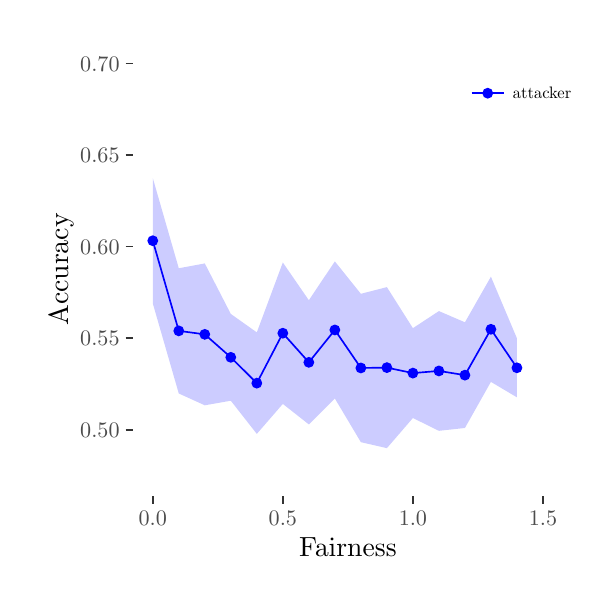
\begin{tikzpicture}[x=1pt,y=1pt]
\definecolor{fillColor}{RGB}{255,255,255}
\path[use as bounding box,fill=fillColor,fill opacity=0.00] (0,0) rectangle (198.74,198.74);
\begin{scope}
\path[clip] (  0.00,  0.00) rectangle (198.74,198.74);
\definecolor{drawColor}{RGB}{255,255,255}
\definecolor{fillColor}{RGB}{255,255,255}

\path[draw=drawColor,line width= 0.6pt,line join=round,line cap=round,fill=fillColor] ( -0.00,  0.00) rectangle (198.74,198.74);
\end{scope}
\begin{scope}
\path[clip] ( 38.16, 29.45) rectangle (193.24,193.24);
\definecolor{fillColor}{RGB}{0,0,255}

\path[fill=fillColor] ( 45.21,121.75) circle (  1.96);

\path[fill=fillColor] ( 54.60, 89.18) circle (  1.96);

\path[fill=fillColor] ( 64.00, 87.92) circle (  1.96);

\path[fill=fillColor] ( 73.40, 79.62) circle (  1.96);

\path[fill=fillColor] ( 82.80, 70.29) circle (  1.96);

\path[fill=fillColor] ( 92.20, 88.34) circle (  1.96);

\path[fill=fillColor] (101.60, 77.81) circle (  1.96);

\path[fill=fillColor] (111.00, 89.51) circle (  1.96);

\path[fill=fillColor] (120.40, 75.77) circle (  1.96);

\path[fill=fillColor] (129.80, 75.90) circle (  1.96);

\path[fill=fillColor] (139.20, 73.92) circle (  1.96);

\path[fill=fillColor] (148.60, 74.70) circle (  1.96);

\path[fill=fillColor] (158.00, 73.18) circle (  1.96);

\path[fill=fillColor] (167.39, 89.75) circle (  1.96);

\path[fill=fillColor] (176.79, 75.83) circle (  1.96);
\definecolor{drawColor}{RGB}{0,0,255}

\path[draw=drawColor,line width= 0.6pt,line join=round] ( 45.21,121.75) --
	( 54.60, 89.18) --
	( 64.00, 87.92) --
	( 73.40, 79.62) --
	( 82.80, 70.29) --
	( 92.20, 88.34) --
	(101.60, 77.81) --
	(111.00, 89.51) --
	(120.40, 75.77) --
	(129.80, 75.90) --
	(139.20, 73.92) --
	(148.60, 74.70) --
	(158.00, 73.18) --
	(167.39, 89.75) --
	(176.79, 75.83);
\definecolor{fillColor}{RGB}{0,0,255}

\path[fill=fillColor,fill opacity=0.20] ( 45.21,144.40) --
	( 54.60,111.80) --
	( 64.00,113.55) --
	( 73.40, 95.30) --
	( 82.80, 88.63) --
	( 92.20,113.89) --
	(101.60,100.25) --
	(111.00,114.28) --
	(120.40,102.57) --
	(129.80,104.99) --
	(139.20, 90.15) --
	(148.60, 96.33) --
	(158.00, 92.28) --
	(167.39,108.75) --
	(176.79, 86.50) --
	(176.79, 65.16) --
	(167.39, 70.75) --
	(158.00, 54.09) --
	(148.60, 53.06) --
	(139.20, 57.69) --
	(129.80, 46.80) --
	(120.40, 48.96) --
	(111.00, 64.74) --
	(101.60, 55.38) --
	( 92.20, 62.79) --
	( 82.80, 51.95) --
	( 73.40, 63.94) --
	( 64.00, 62.28) --
	( 54.60, 66.56) --
	( 45.21, 99.10) --
	cycle;
\end{scope}
\begin{scope}
\path[clip] (  0.00,  0.00) rectangle (198.74,198.74);
\definecolor{drawColor}{gray}{0.30}

\node[text=drawColor,anchor=base east,inner sep=0pt, outer sep=0pt, scale=  0.80] at ( 33.21, 50.68) {0.50};

\node[text=drawColor,anchor=base east,inner sep=0pt, outer sep=0pt, scale=  0.80] at ( 33.21, 83.77) {0.55};

\node[text=drawColor,anchor=base east,inner sep=0pt, outer sep=0pt, scale=  0.80] at ( 33.21,116.86) {0.60};

\node[text=drawColor,anchor=base east,inner sep=0pt, outer sep=0pt, scale=  0.80] at ( 33.21,149.95) {0.65};

\node[text=drawColor,anchor=base east,inner sep=0pt, outer sep=0pt, scale=  0.80] at ( 33.21,183.04) {0.70};
\end{scope}
\begin{scope}
\path[clip] (  0.00,  0.00) rectangle (198.74,198.74);
\definecolor{drawColor}{gray}{0.20}

\path[draw=drawColor,line width= 0.6pt,line join=round] ( 35.41, 53.44) --
	( 38.16, 53.44);

\path[draw=drawColor,line width= 0.6pt,line join=round] ( 35.41, 86.53) --
	( 38.16, 86.53);

\path[draw=drawColor,line width= 0.6pt,line join=round] ( 35.41,119.62) --
	( 38.16,119.62);

\path[draw=drawColor,line width= 0.6pt,line join=round] ( 35.41,152.71) --
	( 38.16,152.71);

\path[draw=drawColor,line width= 0.6pt,line join=round] ( 35.41,185.80) --
	( 38.16,185.80);
\end{scope}
\begin{scope}
\path[clip] (  0.00,  0.00) rectangle (198.74,198.74);
\definecolor{drawColor}{gray}{0.20}

\path[draw=drawColor,line width= 0.6pt,line join=round] ( 45.21, 26.70) --
	( 45.21, 29.45);

\path[draw=drawColor,line width= 0.6pt,line join=round] ( 92.20, 26.70) --
	( 92.20, 29.45);

\path[draw=drawColor,line width= 0.6pt,line join=round] (139.20, 26.70) --
	(139.20, 29.45);

\path[draw=drawColor,line width= 0.6pt,line join=round] (186.19, 26.70) --
	(186.19, 29.45);
\end{scope}
\begin{scope}
\path[clip] (  0.00,  0.00) rectangle (198.74,198.74);
\definecolor{drawColor}{gray}{0.30}

\node[text=drawColor,anchor=base,inner sep=0pt, outer sep=0pt, scale=  0.80] at ( 45.21, 18.99) {0.0};

\node[text=drawColor,anchor=base,inner sep=0pt, outer sep=0pt, scale=  0.80] at ( 92.20, 18.99) {0.5};

\node[text=drawColor,anchor=base,inner sep=0pt, outer sep=0pt, scale=  0.80] at (139.20, 18.99) {1.0};

\node[text=drawColor,anchor=base,inner sep=0pt, outer sep=0pt, scale=  0.80] at (186.19, 18.99) {1.5};
\end{scope}
\begin{scope}
\path[clip] (  0.00,  0.00) rectangle (198.74,198.74);
\definecolor{drawColor}{RGB}{0,0,0}

\node[text=drawColor,anchor=base,inner sep=0pt, outer sep=0pt, scale=  1.00] at (115.70,  7.70) {Fairness};
\end{scope}
\begin{scope}
\path[clip] (  0.00,  0.00) rectangle (198.74,198.74);
\definecolor{drawColor}{RGB}{0,0,0}

\node[text=drawColor,rotate= 90.00,anchor=base,inner sep=0pt, outer sep=0pt, scale=  1.00] at ( 14.59,111.34) {Accuracy};
\end{scope}
\begin{scope}
\path[clip] (  0.00,  0.00) rectangle (198.74,198.74);
\definecolor{fillColor}{RGB}{255,255,255}

\path[fill=fillColor] (154.75,163.56) rectangle (200.72,190.16);
\end{scope}
\begin{scope}
\path[clip] (  0.00,  0.00) rectangle (198.74,198.74);
\definecolor{fillColor}{RGB}{0,0,255}

\path[fill=fillColor] (166.24,175.06) circle (  1.96);
\end{scope}
\begin{scope}
\path[clip] (  0.00,  0.00) rectangle (198.74,198.74);
\definecolor{drawColor}{RGB}{0,0,255}

\path[draw=drawColor,line width= 0.6pt,line join=round] (160.46,175.06) -- (172.02,175.06);
\end{scope}
\begin{scope}
\path[clip] (  0.00,  0.00) rectangle (198.74,198.74);
\definecolor{drawColor}{RGB}{0,0,0}

\node[text=drawColor,anchor=base west,inner sep=0pt, outer sep=0pt, scale=  0.60] at (175.28,172.99) {attacker};
\end{scope}
\end{tikzpicture}
